% !TeX encoding = UTF-8 Unicode
% !TeX root = main.tex
% !TeX TS-program = pdflatex
%% (При смене движка необходимо удалить вспомогательные файлы *.aux *.brf *.log *.out *.synctex.gz *.toc)

\documentclass{thesisby}
\usepackage{etoolbox,ifxetex,ifluatex}
\usepackage[unicode,hypertexnames=false]{hyperref}

%%% Проверка используемого TeX-движка %%%
\ifboolexpr{bool{xetex} or bool{luatex}}{%
  \usepackage{fontspec}
  \PassOptionsToPackage{no-math}{fontspec}     % https://tex.stackexchange.com/a/26295/104425
  \usepackage{polyglossia}%[2014/05/21]        % Поддержка многоязычности

  % fonts and languages
  \defaultfontfeatures{Ligatures=TeX,Mapping=tex-text}

  \setmainlanguage[babelshorthands = true]{russian}
  \setotherlanguage{english}

  \setmainfont{Times New Roman}
  \setmonofont{Courier New}
  \setsansfont{Arial}

  \newfontfamily\cyrillicfont[Script=Cyrillic]{Times New Roman}
  \newfontfamily\cyrillicfontsf[Script=Cyrillic]{Arial}
  \newfontfamily\cyrillicfonttt[Script=Cyrillic]{Courier New}

  \newfontfamily\englishfont{Times New Roman}
  \newfontfamily\englishfontsf{Arial}
  \newfontfamily\englishfonttt{Courier New}

  \renewcommand{\UrlFont}{\small\rmfamily\tt}
}{%
  \usepackage[T1,T2A]{fontenc}
  \usepackage[utf8]{inputenc}
  \usepackage[english, russian]{babel}
  \usepackage{csquotes}
  \IfFileExists{pscyr.sty}{\usepackage{pscyr}}{}  % Подключение pscyr
}

% Для борьбы с переполнениями за счет разреженных слов в абзаце
\emergencystretch=25pt

\usepackage{enumitem}

\usepackage[
    language = auto,        % Получение языка из babel.
    autolang = other,       % Многоязычная библиография.
    defernumbers = true,    % Раздельная нумерация.
    style = gost-numeric,
    maxnames = 10,
    movenames = false,
    sorting = ynt
]{biblatex} % To load multiple bib files.

% Библиографический список в соответствии с ГОСТ.
\makeatletter
\ltx@iffilelater{biblatex-gost.def}{2017/02/01}%
{\toggletrue{bbx:gostbibliography}%
    \renewcommand*{\revsdnamepunct}{\addcomma}}{}
\makeatother

% Общий список.
\addbibresource{references.bib}

% Список публикаций соискателя.
\addbibresource{references.bib}
\DeclareSourcemap{
    \maps[datatype=bibtex, overwrite]{
        \map{
            \perdatasource{references.bib}
            \step[fieldset=KEYWORDS, fieldvalue=ys, append]
        }
    }
}

% Счётчики.
\usepackage[figure,table]{totalcount}   % Счётчик рисунков и таблиц.
\usepackage{totcount}                   % Пакет создания счётчиков на основе последнего номера подсчитываемого элемента (может требовать дважды компилировать документ).
\AtEveryBibitem{\stepcounter{citenum}\stepcounter{citenum_my}}

\usepackage{totpages}
\usepackage[abspage, user, lastpage]{zref}

\usepackage{microtype}

%for lists
\usepackage[ampersand]{easylist}
\ListProperties(Hide=100, Hang=false, Margin=0mm, Indent1=10.5mm, Indent2=15mm, Style*=-- ,
Style2*=$\bullet$ ,Style3*=$\circ$ ,Style4*=\tiny$\blacksquare$ )

\newenvironment{easylistNum}{
    \begin{easylist}
        \ListProperties(Hide1=0, Hang=false, Margin=0mm, Indent1=10.5mm, Indent2=15mm, Start1=1, Style*=, FinalMark={)})}
        {\ListProperties(Hide=100, Hang=false, Margin=0mm, Indent1=10.5mm, Indent2=15mm, Style*=-- , Style2*=$\bullet$ ,Style3*=$\circ$ ,Style4*=\tiny$\blacksquare$ )
    \end{easylist}}

\usepackage{amsmath, amssymb, amsfonts}
\usepackage{mathtools} % Use \rcases
\usepackage{longtable, array}
\usepackage{graphicx, epsfig}
\usepackage{tabularx}

\usepackage{algorithm}        % Для вставки псевдокода
\usepackage{algpseudocode}    % Для вставки псевдокода

% Русская традиция начертания греческих букв
\usepackage{upgreek} % Прямые греческие ради русской традиции (в формулах записывается \alpha как \upalpha и т.д.)

\usepackage{siunitx} % For Celsium sign only

\usepackage{tikz} % Language for producing vector graphics

\begin{document}

% Регистрируем счётчики в системе "totcount".
\regtotcounter{totalcount@table}
\regtotcounter{totalcount@figure}
\regtotcounter{TotPages}
\regtotcounter{textpages}

% Вычисление страниц только с текстом.
\makeatletter
\def\textpages{\number\numexpr\zref@extract{lastpagetocount}{abspage}-\zref@extract{firstpagetocount}{abspage}+1\relax}
\makeatother

\newtotcounter{textpages}
\setcounter{textpages}{\textpages}

% Вычисление количества источников.
\newtotcounter{citenum}
\newtotcounter{citenum_my}

\hypersetup{
    pdftitle = {РАЗРАБОТКА И РЕАЛИЗАЦИЯ ЭФФЕКТИВНОГО АЛГОРИТМА ПЛАНИРОВАНИЯ ПРОИЗВОДСТВА},
    pdfauthor = {Ситковец Яна Сергеевна},
    pdfsubject = {Диссертация},
    pdfkeywords = {ТеХ, диссертация}
}

% !TEX encoding = UTF-8 Unicode
\begin{titlepage}

    \begin{center} \bfseries
        % Национальная академия наук Беларуси\\
        \bigskip
        % {Учреждение образования}
        \medskip

        {БРЕСТСКИЙ ГОСУДАРСТВЕННЫЙ ТЕХНИЧЕСКИЙ УНИВЕРСИТЕТ}
    \end{center}
    \vspace{1cm}

    \noindent УДК 004.032.26 \\
    \vspace{1cm}

    \begin{center}
        {Ситковец \\ Яна Сергеевна}\\
        \vspace{1cm}

        {\bfseries РАЗРАБОТКА И РЕАЛИЗАЦИЯ ЭФФЕКТИВНОГО АЛГОРИТМА ПЛАНИРОВАНИЯ ПРОИЗВОДСТВА}\\
        \vspace{2cm}
        Диссертация на соискание ученой степени\\
        магистра технических наук\\
        \bigskip

        по специальности 7-06-0611-03 -- Искусственный интеллект
    \end{center}
    \vspace{3cm}

    \begin{tabbing}
        \hspace{8cm} \= \kill \>
        Научный руководитель \+ \\
        кандидат технических наук, \\будущий доцент\\
        Иванюк Д. С.
    \end{tabbing}


    \ifdefined\dissertationversion
        \vspace{3cm}
        \begin{center}
            \bfseries v\dissertationversion
        \end{center}
        \vspace{3cm}
    \else
        \vspace{5cm}
    \fi

    \begin{center}
        \bfseries Брест 2025
    \end{center}

\end{titlepage}


\tableofcontents

\zlabel{firstpagetocount}

\chapter*{Введение}
\addcontentsline{toc}{chapter}{Введение}

В условиях стремительного развития технологий и глобализации рынка, оптимизация производственных процессов становится одной из ключевых задач для предприятий, стремящихся сохранить конкурентоспособность и увеличить свою долю на рынке. Особое внимание в этом контексте заслуживает оптимизация фасовочных линий, которые играют критическую роль в производственных цепочках множества отраслей — от пищевой и фармацевтической до косметической и химической. Эффективная работа фасовочных линий не только влияет на объемы производства, но и определяет качество конечного продукта, что в свою очередь имеет прямое отношение к удовлетворенности потребителей и репутации компании.

Оптимизация фасовочных линий включает в себя множество аспектов: от сокращения времени простоя оборудования до повышения точности дозирования и улучшения логистики. Современные предприятия сталкиваются с необходимостью адаптации к быстро меняющимся условиям рынка, что требует гибкости в производственных процессах. Эффективное управление ресурсами и планирование позволяет значительно снизить затраты, повысить производительность и улучшить качество продукции. Таким образом, задача оптимизации становится не просто желательной, а жизненно необходимой для достижения устойчивого роста и развития бизнеса.

Среди современных инструментов, используемых для решения задач оптимизации, особое место занимают программные решения, такие как Timefold Solver. Этот инструмент представляет собой мощный планировщик, который позволяет моделировать и оптимизировать производственные процессы с учетом множества факторов, включая ограничения по ресурсам, временные рамки и требования к качеству. Timefold Solver использует алгоритмы оптимизации, способные находить эффективные решения даже в сложных ситуациях с большим количеством переменных. Его применение позволяет значительно сократить время на планирование и повысить точность прогнозов, что в свою очередь способствует более рациональному использованию ресурсов и снижению операционных затрат.

Таким образом, данная магистерская диссертация будет посвящена исследованию методов и инструментов оптимизации фасовочных линий, с акцентом на использование Timefold Solver как примера современного подхода к решению задач планирования. В рамках работы будут рассмотрены основные принципы работы фасовочных линий, выявлены ключевые проблемы, с которыми сталкиваются предприятия, а также предложены рекомендации по их решению с использованием современных технологий. Ожидается, что результаты данного исследования смогут внести значительный вклад в развитие практических аспектов управления производственными процессами и оптимизации ресурсов на предприятиях различных отраслей.
\chapter*{ОБЩАЯ ХАРАКТЕРИСТИКА РАБОТЫ}
\addcontentsline{toc}{chapter}{ОБЩАЯ ХАРАКТЕРИСТИКА РАБОТЫ}
\label{ch:target}

Тема диссертации соответствует приоритетному направлению научно-технической деятельности согласно пункту 1 перечня приоритетных направлений научной, научно-технической и инновационной деятельности на 2021-2025 годы (Указ Президента Республики Беларусь от 07 мая 2020 г. № 156).

\medskip  % примерно 6pt
\bigskip  % примерно 12pt

\noindent \textbf{Цель работы:}

Улучшение эффективности производства за счет минимизации времени выполнения задач и оптимального использования ресурсов. Определить возможные улучшения и дальнейшие направления исследования. Оценить влияние оптимизации на производительность, время выполнения задач и использование ресурсов.

\noindent \textbf{Задачи:}
\begin{enumerate}
    \item Анализ существующих процессов:
Изучить текущие методы и процессы фасовки.
Определение ключевых ограничений и требований, таких как время, ресурсы, оборудование и персонал. Проведение сравнения с существующими методами планирования.
    \item  Моделирование задачи планирования:
Создать модель задачи планирования в Timefold Solver, учитывая специфику фасовки того или иного товара. Определить переменные, ограничения и целевую функцию для оптимизации.
    \item Разработка алгоритма оптимизации:
Использовать современные инструменты для решения задач оптимизации, для поиска наилучшего расписания.
Оптимизировать расписание с учетом минимизации времени выполнения задач, использования ресурсов и обеспечения высокой производительности.
    \itemРеализация модели:
Реализовать разработанный алгоритм на Java с использованием Timefold Solver.
    \item Тестирование результатов:\
Протестировать эффективность разработанного алгоритма.
\item Внедрение и рекомендации:\
Предложить рекомендации по внедрению разработанного планирования в реальном производстве.
\end{enumerate}

\vspace{6mm}


\textit{Объектом исследования} являются фасовочные линии на производстве.

\vspace{6mm}

\textit{Предметом исследования} выступают методы и алгоритмы оптимизации в соврменных системах планирования.

\vspace{6mm}

\noindent \textbf{Положения выносимые на защиту}
\begin{enumerate}
    \item Программная система составляюшая план фасовки производственного заказа глазированных сырков.
    \item Анализ результатов тестирования работы системы.
\end{enumerate}

\vspace{6mm}

\noindent \textbf{Личный вклад соискателя}\\
\indent Разработка программной системы, получение результатов оценки планирования работы фасовочных линий.

\vspace{6mm}

\textit{Научная новизна} состоит в оценке эффективности использования современных систем планирования.

\vspace{6mm}

\noindent \textbf{Структура и объем диссертации}\\


\chapter{ ГЛАВА 1. Задача оптимизации}
\label{ch:chapter2}

\section{Процесс оптимизации}

Многие научные и инженерные дисциплины основаны на оптимизации. B физике системы стремятся к состоянию с наименьшей энергией в соответствии с законами природы. B бизнесе корпорации нацелены на максимальную стоимость акций. B биологии с большей вероятностью выживают более адаптивные организмы. Данная работа посвящена оптимизации с инженерной точки зрения, для которой целью является разработка системы, оптимизирующих набор показателей с учетом ограничений.

Типичный процесс оптимизации инженерного проектирования показан на рис. \ref{fig:diagram_1} Роль конструктора заключается в предоставлении технического задания, которое детализирует параметры, константы, цели и ограничения. Конструктор отвечает за постановку задачи и количественную оценку достоинств потенциальных проектов. Он также обычно предоставляет базовый проект или начальную точку проектирования для алгоритма оптимизации.

\begin{figure}[ht]
 \centering
		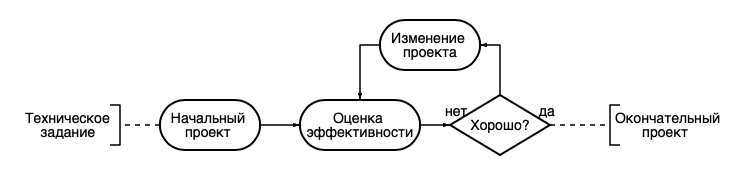
\includegraphics[height = 3 cm, keepaspectratio]{../assets/images/1_1_1diagram.png}
		\caption{ Процесс оптимизации }
		\label{fig:diagram_1}
	\end{figure}

Алгоритм оптимизации используется для постепенного улучшения проекта до тех пор, пока проект больше не может быть улучшен или пока не будет затрачено запланированное время либо превышена предельно допустимая стоимость. Конструктор несет ответственность за анализ результатов процесса оптимизации, чтобы обеспечить его пригодность для конечного применения. Неправильные спецификации в постановке задачи, плохой начальный проект и неправильно реализованные или неподходящие алгоритмы оптимизации могут привести к неоптимальным или опасным проектам.

Есть несколько преимуществ оптимизации подхода к проектированию. Прежде всего, процесс оптимизации обеспечивает систематическую, логичную процедуру проектирования. При ее правильном соблюдении алгоритмы оптимизации могут уменьшить вероятность ошибки человека при проектировании. Интуиция в инженерном проектировании может ввести в заблуждение; намного лучше оптимизировать данные. Оптимизация может ускорить процесс проектирования, особенно когда процедура может быть написана один раз, а затем повторно применена к другим задачам. Традиционные инженерные методы часто визуализируются и обосновываются людьми в двух или трех измерениях. B то же время современные методы оптимизации могут применяться к задачам с миллионами переменных и ограничений.
   
Есть также проблемы, связанные с использованием оптимизации для проектирования. Мы обычно ограничены в наших вычислительных ресурсах и времени, и поэтому наши алгоритмы должны быть избирательными в том, как они исследуют пространство проектных параметров. По сути, алгоритмы оптимизации ограничены способностью конструктора формулировать задачу. B некоторых случаях алгоритм оптимизации может использовать ошибки моделирования или найти решение, которое не позволяет адекватно решить поставленную задачу. Когда алгоритм приводит к оптимальному проекту, который противоречит интуиции, его может быть трудно интерпретировать. Другое ограничение заключается в том, что многие алгоритмы оптимизации не всегда гарантируют получение оптимальных проектов. 

\section{Математическое определение задачи оптимизации}

Основная задача оптимизации формулируется следующим образом:

\begin{equation}
  \min_{x} \, f(x)
  \label{eq:taskOptimizationMin}
\end{equation}

\begin{center}
при условии, что $x \in X$
\end{center}

Здесь $x$ — расчетная точка (design point). Расчетная точка мохет быть представлена как вектор значений, соответствующих различным расчетным переменным (design variables). Расчетная точка в $n$-мерном пространстве записывается следующим образом:

\begin{equation}
    [x_1,x_2,...,x_n],
	\label{eq:arrayX}
\end{equation}

где $i$-я расчетная переменная обозначена $x_i$. Элементы в этом векторе можно регулировать, чтобы минимизировать целевую функцию $f$. Любое значение $x$ из всех точек в допустимом множестве $F$, которое минимизирует целевую функцию, называется решением или точкой минимума. Конкретное решение записывается как $x^*$. Пример задачи одномерной оптимизации показан на рис. \ref{fig:figure_1}

\begin{figure}[ht]
 \centering
		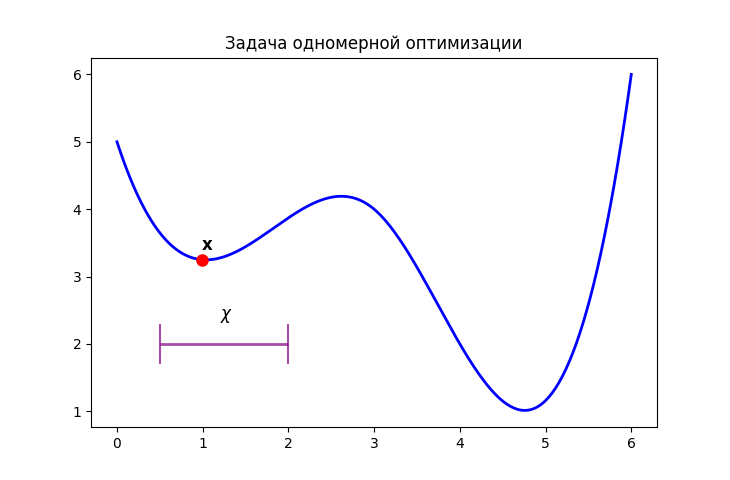
\includegraphics[height =7 cm, keepaspectratio]{../assets/images/Figure_1.png}
		\caption{Минимум является лучшим вариантом в возможном наборе —
вне допустимой области могут существовать точки с более низкими значениями
}
\label{fig:figure_1}
	\end{figure}

Эта формулировка является общей, т.е. любая задача оптимизации может быть переписана в соответствии с уравнением \eqref{eq:taskOptimizationMin}. B частности, задачу

\begin{equation}
  \min_{x} \, f(x) 
\end{equation}

\begin{center}
при условии, что $x \in X$
\end{center}

можно переформулировать так:

\begin{equation}
  \max_{x} \, -f(x) 
  \label{eq:TaskOptimizationMax}
\end{equation}

 \begin{center}
 при условии, что $x \in X$
 \end{center}
 
Задача в новой формулировке имеет тот же самый набор решений. Моделирование инженерных задач в рамках этой математической формулировки может быть сложной задачей. То, как формулируется задача оптимизации, может сделать процесс решения простым или сложным. Следует задаться вопросом какой алгоритм лучше. Если один алгоритм работает лучше, чем другой алгоритм для одного класса задач, то он будет работать хуже для другого класса задач. Чтобы многие алгоритмы оптимизации работали эффективно, в целевой функции должна быть некоторая регулярность, например липшиц-непрерывность или выпуклость. 

\section{Ограничения}

Многие задачи имеют ограничения. Каждое ограничение выделяет множество возможных решений, и в совокупности ограничения определяют допустимое множество  $F$. Допустимые расчетные точки не нарушают никаких ограничений. Например, рассмотрим следующую проблему оптимизации:

\begin{equation}
\min_{x_1, x_2} f(x_1, x_2)
\label{eq:taskOptimizationX1X2}
\end{equation}


 \begin{center}
 при условии, что 
\begin{equation}
  \begin{aligned}
    x_1 &\geq  \\
    x_2 &\geq 0  \\
    x_1 + x_2 &\leq 1
  \end{aligned}
  \label{eq:inequalities}
\end{equation}
\end{center}

Допустимое множество изображено на рис. \ref{fig:figure_2}

\begin{figure}[ht]
 \centering
		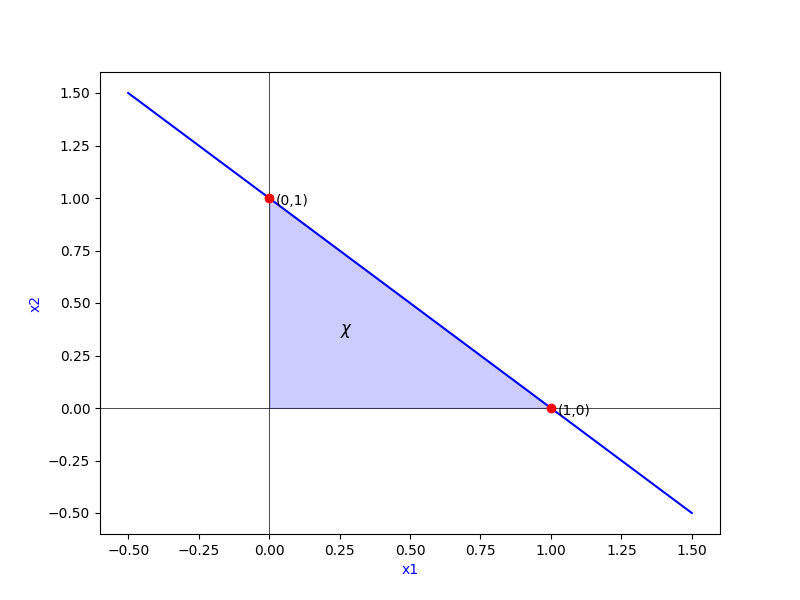
\includegraphics[height = 7 cm, keepaspectratio]{../assets/images/Figure_2.png}
		\caption{Допустимое множество F, заданное неравенствами \eqref{eq:inequalities}}
		\label{fig:figure_2}
	\end{figure}
    
Ограничения обычно записываются с помощью знаков $\leq$, $\geq$ или $=$. Если ограничения включают знаки $<$ или $>$ (т.е. строгие неравенства), то допустимое множество не включает границу ограничений. Потенциальная проблема, которая может возникнуть без учета границы иллюстрируется следующей задачей:


\begin{equation}
  \min_{x} \, x 
  \label{eq:taskOptimizationMin1}
\end{equation}

 \begin{center}
 при условии, что $x>1$
 \end{center}

 Допустимое множество показано на рис. \ref{fig:figure_3} Точка $x = 1$ меньше любого $x$, превышающего единицу, но значение $x = 1$ недопустимо. Можно выбрать любой $x$, произвольно близкий к единице, но превышающей ее, и независимо от того, что выбирать, всегда можно найти бесконечное количество значений, которые расположены еще ближе к единице. Необходимо констатировать, что задача не имеет решения. Чтобы избежать таких проблем, часто лучше включать границу ограничений в допустимое множество.


\begin{figure}[ht]
 \centering
		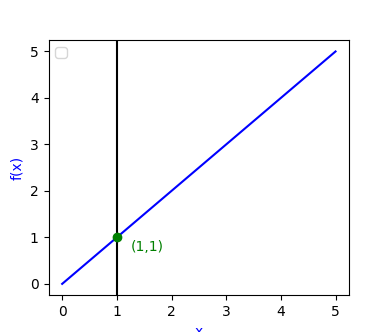
\includegraphics[height = 5 cm, keepaspectratio]{../assets/images/Figure_3.png}
		\caption{ Задача \eqref{eq:taskOptimizationMin1} не имеет решения, поскольку граница ограничения недопустима }
		\label{fig:figure_3}
	\end{figure}
    
\section{Критические точки}

На рис. 2.4.1 ~\ref{fig:figure_4} показана одномерная функция $f(x)$ с несколькими помеченными критическими точками, в которых производная равна нулю и которые представляют интерес при обсуждении задач оптимизации. При минимизации функции $f$ желательно найти точку глобального минимума, т.е. значение $x$, в котором значение $f(x)$ является минимальным. Функция может иметь не более одного глобального минимума, но может иметь несколько точек глобального минимума.

Как правило, трудно доказать, что данная точка-кандидат является точкой глобального минимума. Часто лучшее, что можно сделать, это проверить, соответствует ли она локальному минимуму. Точка $x^*$ является точкой локального минимума, если существует число $\delta > 0$ такое, что $f(x^*) \leq f(x)$ для всех $x$, удовлетворяющих условию $| x - x^*| < \delta$. B многомерном контексте это определение сводится к существованию числа $\delta > 0$ такого, что $f(x^*) \leq f (x)$ для всех $x$, удовлетворяющих условию $||x - x^*|| < \delta$.
На рис. \ref{fig:figure_4} показаны два типа локальных минимумов: сильный и слабый. Точка сильного локального минимума, которая также называется точкой строгого локального минимума, — это точка, которая однозначно минимизирует $f$ в окрестности. Иначе говоря, точка $x^*$ является точкой строгого локального минимума, если существует число $\delta > 0$ такое, что $f(x^*) < f(x)$ всякий раз, когда $x^* \neq x$ и $||x - x^*|| < \delta$. B многомерном контексте это определение сводится к существованию числа $\delta > 0$ такого, что $f(x^*)< f(x)$всякийраз,когда $x^* \neq x$ и $||x - x^*||< \delta$. Точка слабого локального минимума — это точка локального минимума, которая не является точкой сильного локального минимума.

\begin{figure}[ht]
 \centering
		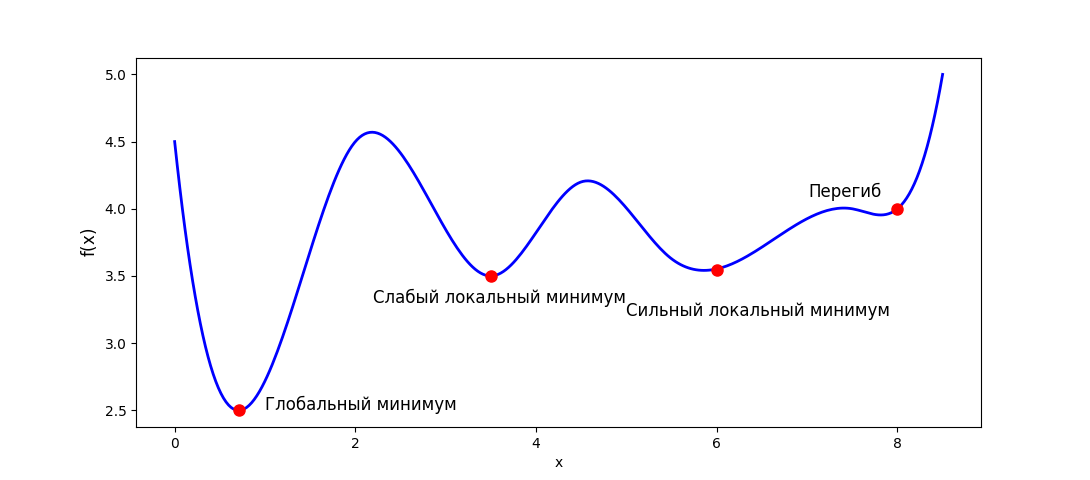
\includegraphics[height =5 cm, keepaspectratio]{../assets/images/Figure_4.png}
		\caption{Примеры критических точек одномерной функции, представляющих интерес для алгоритмов оптимизации (в которых производная равна нулю)
		\label{fig:figure_4}
 }
	\end{figure}
    
Bо всех точках локального и глобального минимума производная непрерывной неограниченной целевой функции равна нулю. Равенство производной нулю — необходимое, но не достаточное условие для локального минимума.
На рис. \ref{fig:figure_4} показана точка перегиба, где производная равна нулю, но эта точка не является точкой локального минимума функции $f$. Точка перегиба — это место, где меняется знак второй производной функции $f$, что соответствует локальному минимуму или максимуму ее первой производной $f '$. Производная в точке перегиба не обязательно равна нулю.

\chapter{ ГЛАВА 2. Задача оптимизации}
\label{ch:chapter2}

\section{Процесс оптимизации}

Многие научные и инженерные дисциплины основаны на оптимизации. B физике системы стремятся к состоянию с наименьшей энергией в соответствии с законами природы. B бизнесе корпорации нацелены на максимальную стоимость акций. B биологии с большей вероятностью выживают более адаптивные организмы. Данная работа посвящена оптимизации с инженерной точки зрения, для которой целью является разработка системы, оптимизирующих набор показателей с учетом ограничений.

Типичный процесс оптимизации инженерного проектирования показан на рис. \ref{fig:diagram_1} Роль конструктора заключается в предоставлении технического задания, которое детализирует параметры, константы, цели и ограничения. Конструктор отвечает за постановку задачи и количественную оценку достоинств потенциальных проектов. Он также обычно предоставляет базовый проект или начальную точку проектирования для алгоритма оптимизации.

\begin{figure}[ht]
 \centering
		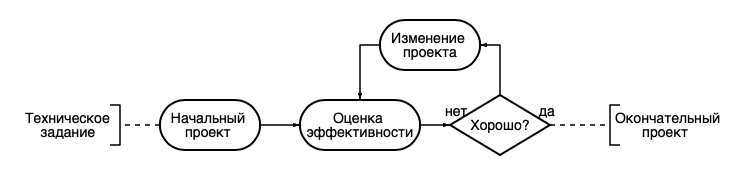
\includegraphics[height = 3 cm, keepaspectratio]{../assets/images/1_1_1diagram.png}
		\caption{ Процесс оптимизации }
		\label{fig:diagram_1}
	\end{figure}

Алгоритм оптимизации используется для постепенного улучшения проекта до тех пор, пока проект больше не может быть улучшен или пока не будет затрачено запланированное время либо превышена предельно допустимая стоимость. Конструктор несет ответственность за анализ результатов процесса оптимизации, чтобы обеспечить его пригодность для конечного применения. Неправильные спецификации в постановке задачи, плохой начальный проект и неправильно реализованные или неподходящие алгоритмы оптимизации могут привести к неоптимальным или опасным проектам.

Есть несколько преимуществ оптимизации подхода к проектированию. Прежде всего, процесс оптимизации обеспечивает систематическую, логичную процедуру проектирования. При ее правильном соблюдении алгоритмы оптимизации могут уменьшить вероятность ошибки человека при проектировании. Интуиция в инженерном проектировании может ввести в заблуждение; намного лучше оптимизировать данные. Оптимизация может ускорить процесс проектирования, особенно когда процедура может быть написана один раз, а затем повторно применена к другим задачам. Традиционные инженерные методы часто визуализируются и обосновываются людьми в двух или трех измерениях. B то же время современные методы оптимизации могут применяться к задачам с миллионами переменных и ограничений.
   
Есть также проблемы, связанные с использованием оптимизации для проектирования. Мы обычно ограничены в наших вычислительных ресурсах и времени, и поэтому наши алгоритмы должны быть избирательными в том, как они исследуют пространство проектных параметров. По сути, алгоритмы оптимизации ограничены способностью конструктора формулировать задачу. B некоторых случаях алгоритм оптимизации может использовать ошибки моделирования или найти решение, которое не позволяет адекватно решить поставленную задачу. Когда алгоритм приводит к оптимальному проекту, который противоречит интуиции, его может быть трудно интерпретировать. Другое ограничение заключается в том, что многие алгоритмы оптимизации не всегда гарантируют получение оптимальных проектов. 

\section{Математическое определение задачи оптимизации}

Основная задача оптимизации формулируется следующим образом:

\begin{equation}
  \min_{x} \, f(x)
  \label{eq:taskOptimizationMin}
\end{equation}

\begin{center}
при условии, что $x \in X$
\end{center}

Здесь $x$ — расчетная точка (design point). Расчетная точка мохет быть представлена как вектор значений, соответствующих различным расчетным переменным (design variables). Расчетная точка в $n$-мерном пространстве записывается следующим образом:

\begin{equation}
    [x_1,x_2,...,x_n],
	\label{eq:arrayX}
\end{equation}

где $i$-я расчетная переменная обозначена $x_i$. Элементы в этом векторе можно регулировать, чтобы минимизировать целевую функцию $f$. Любое значение $x$ из всех точек в допустимом множестве $F$, которое минимизирует целевую функцию, называется решением или точкой минимума. Конкретное решение записывается как $x^*$. Пример задачи одномерной оптимизации показан на рис. \ref{fig:figure_1}

\begin{figure}[ht]
 \centering
		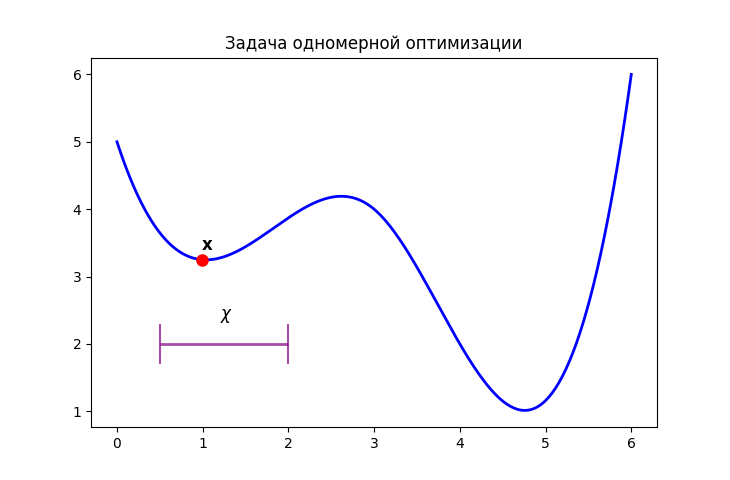
\includegraphics[height =7 cm, keepaspectratio]{../assets/images/Figure_1.png}
		\caption{Минимум является лучшим вариантом в возможном наборе —
вне допустимой области могут существовать точки с более низкими значениями
}
\label{fig:figure_1}
	\end{figure}

Эта формулировка является общей, т.е. любая задача оптимизации может быть переписана в соответствии с уравнением \eqref{eq:taskOptimizationMin}. B частности, задачу

\begin{equation}
  \min_{x} \, f(x) 
\end{equation}

\begin{center}
при условии, что $x \in X$
\end{center}

можно переформулировать так:

\begin{equation}
  \max_{x} \, -f(x) 
  \label{eq:TaskOptimizationMax}
\end{equation}

 \begin{center}
 при условии, что $x \in X$
 \end{center}
 
Задача в новой формулировке имеет тот же самый набор решений. Моделирование инженерных задач в рамках этой математической формулировки может быть сложной задачей. То, как формулируется задача оптимизации, может сделать процесс решения простым или сложным. Следует задаться вопросом какой алгоритм лучше. Если один алгоритм работает лучше, чем другой алгоритм для одного класса задач, то он будет работать хуже для другого класса задач. Чтобы многие алгоритмы оптимизации работали эффективно, в целевой функции должна быть некоторая регулярность, например липшиц-непрерывность или выпуклость. 

\section{Ограничения}

Многие задачи имеют ограничения. Каждое ограничение выделяет множество возможных решений, и в совокупности ограничения определяют допустимое множество  $F$. Допустимые расчетные точки не нарушают никаких ограничений. Например, рассмотрим следующую проблему оптимизации:

\begin{equation}
\min_{x_1, x_2} f(x_1, x_2)
\label{eq:taskOptimizationX1X2}
\end{equation}


 \begin{center}
 при условии, что 
\begin{equation}
  \begin{aligned}
    x_1 &\geq  \\
    x_2 &\geq 0  \\
    x_1 + x_2 &\leq 1
  \end{aligned}
  \label{eq:inequalities}
\end{equation}
\end{center}

Допустимое множество изображено на рис. \ref{fig:figure_2}

\begin{figure}[ht]
 \centering
		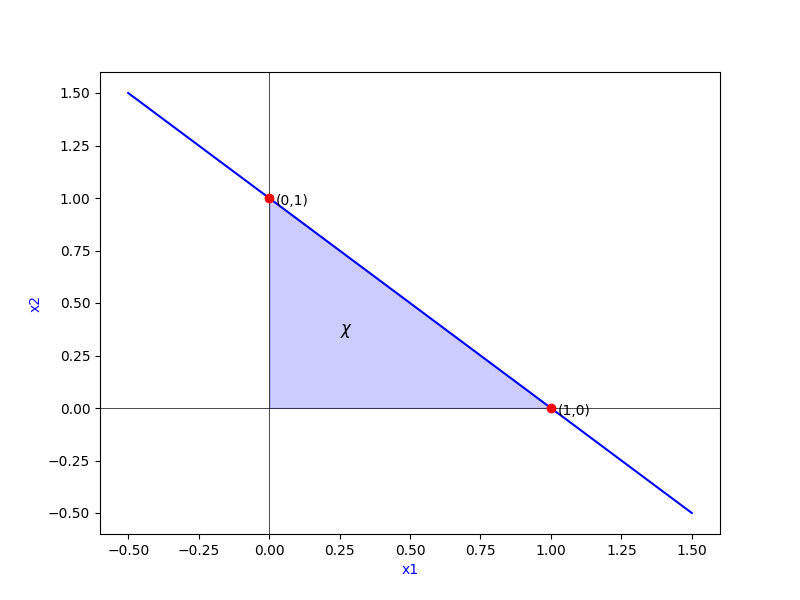
\includegraphics[height = 7 cm, keepaspectratio]{../assets/images/Figure_2.png}
		\caption{Допустимое множество F, заданное неравенствами \eqref{eq:inequalities}}
		\label{fig:figure_2}
	\end{figure}
    
Ограничения обычно записываются с помощью знаков $\leq$, $\geq$ или $=$. Если ограничения включают знаки $<$ или $>$ (т.е. строгие неравенства), то допустимое множество не включает границу ограничений. Потенциальная проблема, которая может возникнуть без учета границы иллюстрируется следующей задачей:


\begin{equation}
  \min_{x} \, x 
  \label{eq:taskOptimizationMin1}
\end{equation}

 \begin{center}
 при условии, что $x>1$
 \end{center}

 Допустимое множество показано на рис. \ref{fig:figure_3} Точка $x = 1$ меньше любого $x$, превышающего единицу, но значение $x = 1$ недопустимо. Можно выбрать любой $x$, произвольно близкий к единице, но превышающей ее, и независимо от того, что выбирать, всегда можно найти бесконечное количество значений, которые расположены еще ближе к единице. Необходимо констатировать, что задача не имеет решения. Чтобы избежать таких проблем, часто лучше включать границу ограничений в допустимое множество.


\begin{figure}[ht]
 \centering
		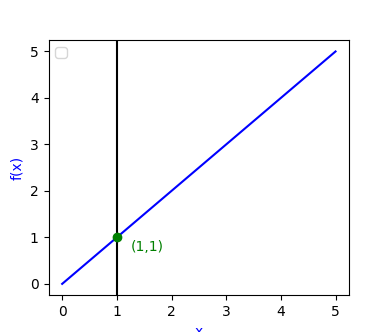
\includegraphics[height = 5 cm, keepaspectratio]{../assets/images/Figure_3.png}
		\caption{ Задача \eqref{eq:taskOptimizationMin1} не имеет решения, поскольку граница ограничения недопустима }
		\label{fig:figure_3}
	\end{figure}
    
\section{Критические точки}

На рис. 2.4.1 ~\ref{fig:figure_4} показана одномерная функция $f(x)$ с несколькими помеченными критическими точками, в которых производная равна нулю и которые представляют интерес при обсуждении задач оптимизации. При минимизации функции $f$ желательно найти точку глобального минимума, т.е. значение $x$, в котором значение $f(x)$ является минимальным. Функция может иметь не более одного глобального минимума, но может иметь несколько точек глобального минимума.

Как правило, трудно доказать, что данная точка-кандидат является точкой глобального минимума. Часто лучшее, что можно сделать, это проверить, соответствует ли она локальному минимуму. Точка $x^*$ является точкой локального минимума, если существует число $\delta > 0$ такое, что $f(x^*) \leq f(x)$ для всех $x$, удовлетворяющих условию $| x - x^*| < \delta$. B многомерном контексте это определение сводится к существованию числа $\delta > 0$ такого, что $f(x^*) \leq f (x)$ для всех $x$, удовлетворяющих условию $||x - x^*|| < \delta$.
На рис. \ref{fig:figure_4} показаны два типа локальных минимумов: сильный и слабый. Точка сильного локального минимума, которая также называется точкой строгого локального минимума, — это точка, которая однозначно минимизирует $f$ в окрестности. Иначе говоря, точка $x^*$ является точкой строгого локального минимума, если существует число $\delta > 0$ такое, что $f(x^*) < f(x)$ всякий раз, когда $x^* \neq x$ и $||x - x^*|| < \delta$. B многомерном контексте это определение сводится к существованию числа $\delta > 0$ такого, что $f(x^*)< f(x)$всякийраз,когда $x^* \neq x$ и $||x - x^*||< \delta$. Точка слабого локального минимума — это точка локального минимума, которая не является точкой сильного локального минимума.

\begin{figure}[ht]
 \centering
		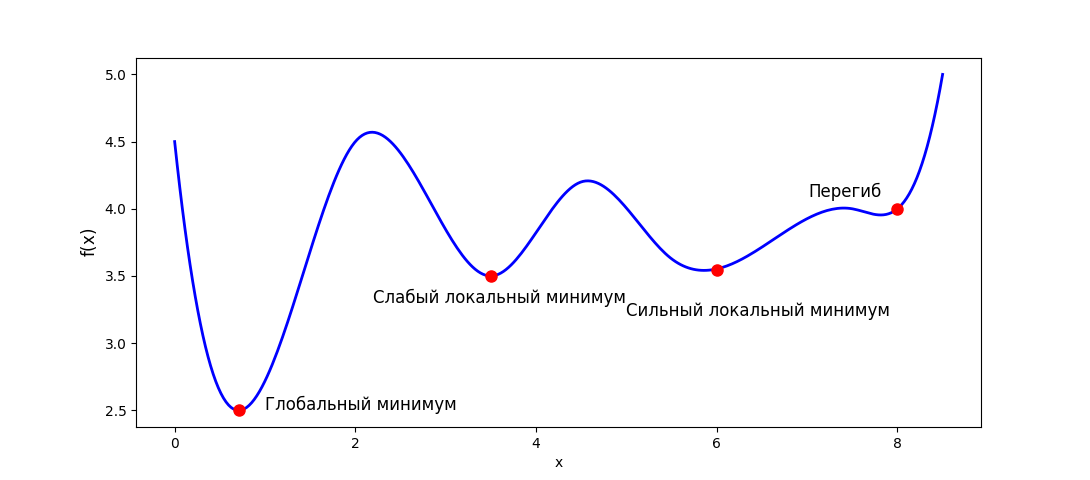
\includegraphics[height =5 cm, keepaspectratio]{../assets/images/Figure_4.png}
		\caption{Примеры критических точек одномерной функции, представляющих интерес для алгоритмов оптимизации (в которых производная равна нулю)
		\label{fig:figure_4}
 }
	\end{figure}
    
Bо всех точках локального и глобального минимума производная непрерывной неограниченной целевой функции равна нулю. Равенство производной нулю — необходимое, но не достаточное условие для локального минимума.
На рис. \ref{fig:figure_4} показана точка перегиба, где производная равна нулю, но эта точка не является точкой локального минимума функции $f$. Точка перегиба — это место, где меняется знак второй производной функции $f$, что соответствует локальному минимуму или максимуму ее первой производной $f '$. Производная в точке перегиба не обязательно равна нулю.


\zlabel{lastpagetocount}

\printbibliography

\end{document}
